\documentclass[a4paper,10pt]{report}
\usepackage[utf8x]{inputenc}
\usepackage{graphicx}
\usepackage{float}
\usepackage{listings}
\usepackage{amsmath}

% Title Page
\title{AST2210 Report 1}
\author{Andreas Ellewsen}

\begin{document}
\maketitle

\section{Assignment}
In short the whole lab is about extracting data from the Hinode database. 
We are also supposed to interpret this data and plot som pictures underways.
Of the things we did we were to include in this report how we did the following 3 exercises:

Exercise 3:
Read into IDL the SOT/BFI synoptic images from Exercise 2.
Compare the images in the various wavelengths. Look for image artifacts. List the
minimum value, maximum value, mean and standard deviation of each image.

Exercise 7:
Extract a few images from the timeseries and determine the average
motion of the limb. Store the average displacement per timestep in the variables
dx and dy. Make an array with this information and correct the time-series for this
drift.

Exercise 8:
Spicules have an apparent motion outwards. Find a good example in the cube cahalign.icube and measure the outward velocity.

\section{Exercise 3}

Here we follow the instructions from Exercise 1 and 2. We're asked to find some values for each of the images we load into IDL.
This is done by using the code we're given in the assignment. The values can be seen in the table below. When comparing the images
we see that there are some dead pixels. There is also a difference in brightness in them as well as the left and right side in each of them. 
The clearest error in all of them is the vertical line in the middle.

\begin{table}[h!]
\center
\begin{tabular}{|l|l|l|l|l|}
\hline
Image			&Max	&Min	&Mean	&Std dev\\
\hline
red cont 6684		&1608	&0	&964.102&63.2199\\
green cont 5550		&1309	&0	&896.604&69.5269\\
blue cont 4504		&1149	&92	&759.703&79.3695\\
G band 4305		&1310	&93	&745.198&67.4408\\
Ca II H line		&1262	&96	&431.999&36.7945\\
CN bandhead 3883	&1973	&20	&1018.62&114.788\\
\hline
\end{tabular}
\caption{Values for all the pictures}
\end{table}

The pictures and the code used to generate all of this are included at the end of the report.




\section{Exercise 7}

Here we do exactly what we're told. Basically copying the code from the assignment. 
We noticed in the last exercise, that the limb of the sun was moving. 
We want to fix this and we do this by looking at the displacement per timestep and store it in the variable dx. 
It is not necessary (like the assigment says) to save anything for dy since there is no change in the y direction.
This as going to make the next exercise easier. 

The code is included at the end of the report.


\section{Exercise 8}

Now that we've got the sun to stand still, we want to measure the velocity of one of the specules.
This was not as easy as expected. I ended up just finding one that was at least a little clear and 
just time the number of frames it took to move a distance of some pixels.
I looked at frame number 115 at position (799,653). I then looked at this spicule until it dissapeared.
This happened at frame 116 when it reached position (784,653). So in 1 frame it moved 15 pixels.
We see from the Hinode data we gathered that the time between frames is 16 seconds

The lecture notes say that for small $p$ we can say that 
\begin{equation}
 p = \frac{a}{r}
\end{equation}
The Hinode data tells us that Hinode has a resolution of 
\begin{equation}
0.0541\frac{arcseconds}{pixel}
\end{equation}
This gives us
$$15\times0.0541arcseconds = tan\frac{r}{1AU}$$
$$r = 15\times0.0541 arcseconds\times 1AU$$
and the velocity of the spicule is thus 
$$\frac{r}{t} = 3.93426302\times10^{-6}\frac{1AU}{16seconds}$$
converting this to familiar units gives
$$\frac{r}{t} \approx 36 784\frac{m}{s}$$

\section{Conclusion}
In conclusion I thought I'd make a list of the things we learned in this lab.
\begin{itemize}
\item How to access the data from Hinode. 
\item How to load this data into IDL.
\item How to look at spesific attributes about each image.
\item How to fix artifacts and other irregularities in one, or many images.
\item How to save these images to the harddrive. 
\item How to load a series of images into Crispex and save this as a movie. 
\item How to force the video to keep a part of the sun at a specific place in the video.
\item Finally we made a guess at the velocity of a spicule.
\end{itemize}

\section{Code}
\subsection{Exercise3}
\lstinputlisting[language=IDL, firstline=1, lastline=42]{oblig1.pro}
\newpage
\subsection{Exercise7}
\lstinputlisting[language=IDL]{oblig1e6.pro}

\newpage
\section{Pictures from Exercise 3}
\begin{figure}[H]
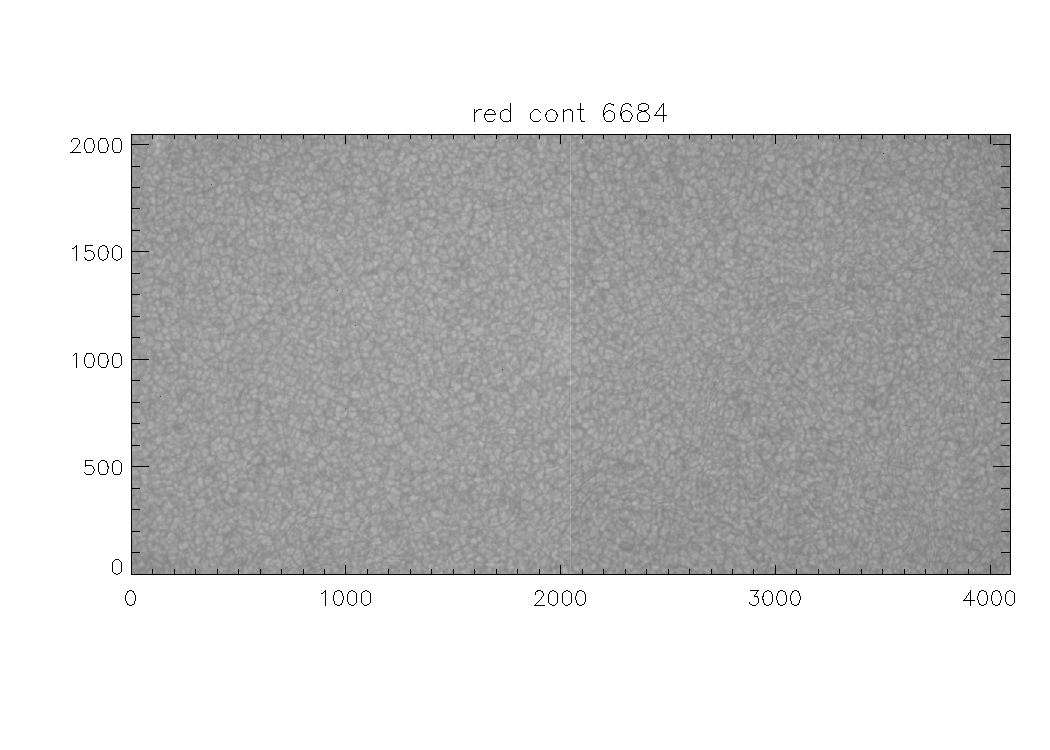
\includegraphics[width=\linewidth]{file0.pdf}
\end{figure}

\begin{figure}[H]
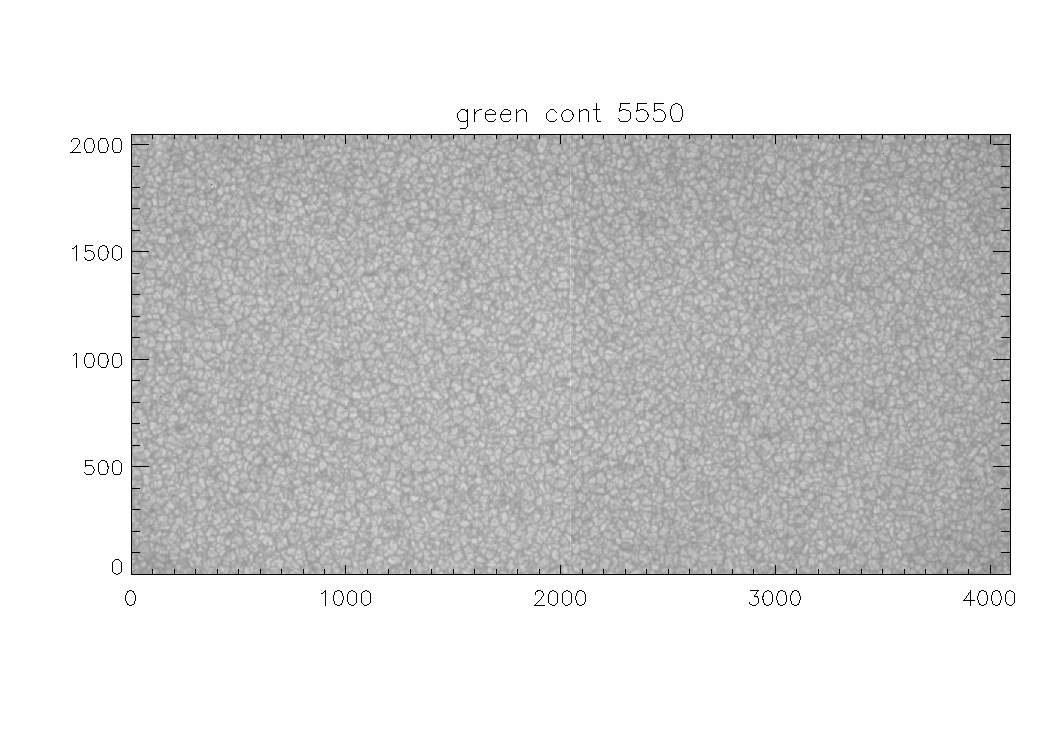
\includegraphics[width=\linewidth]{file1.pdf}
\end{figure}

\begin{figure}[H]
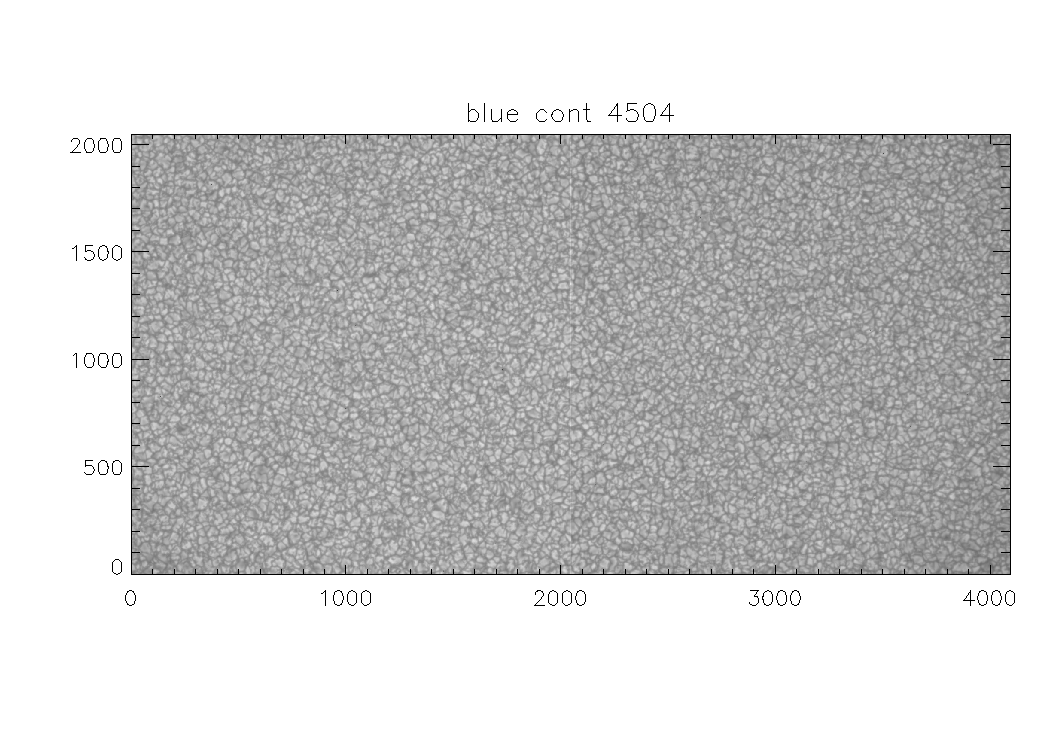
\includegraphics[width=\linewidth]{file2.pdf}
\end{figure}

\begin{figure}[H]
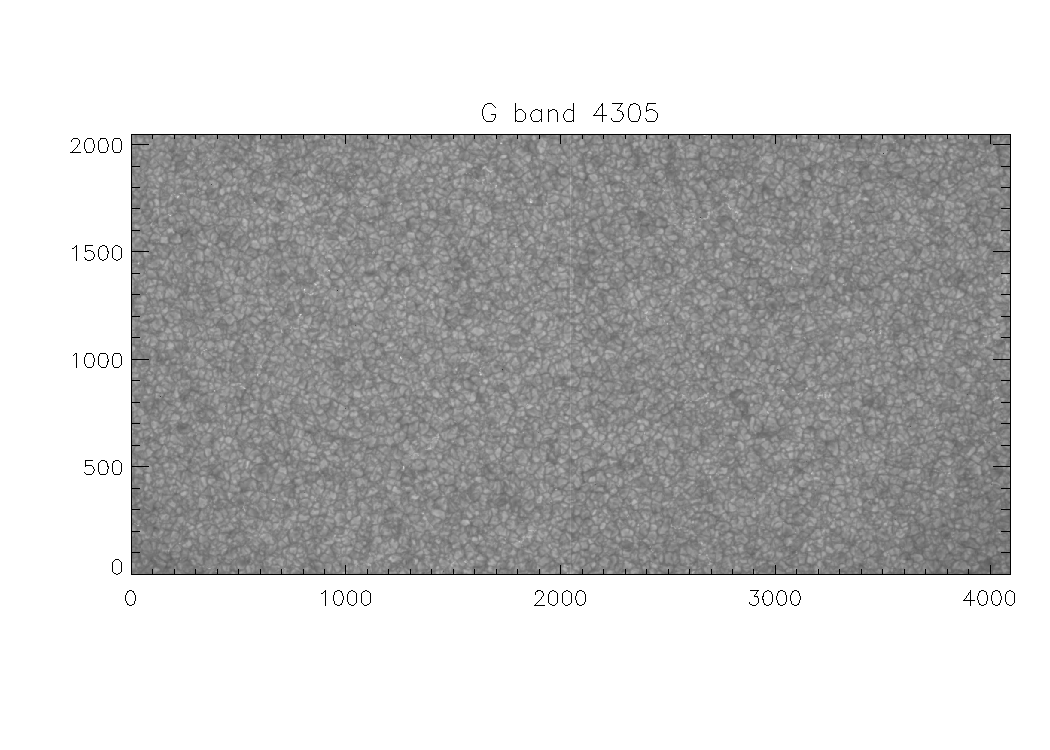
\includegraphics[width=\linewidth]{file3.pdf}
\end{figure}

\begin{figure}[H]
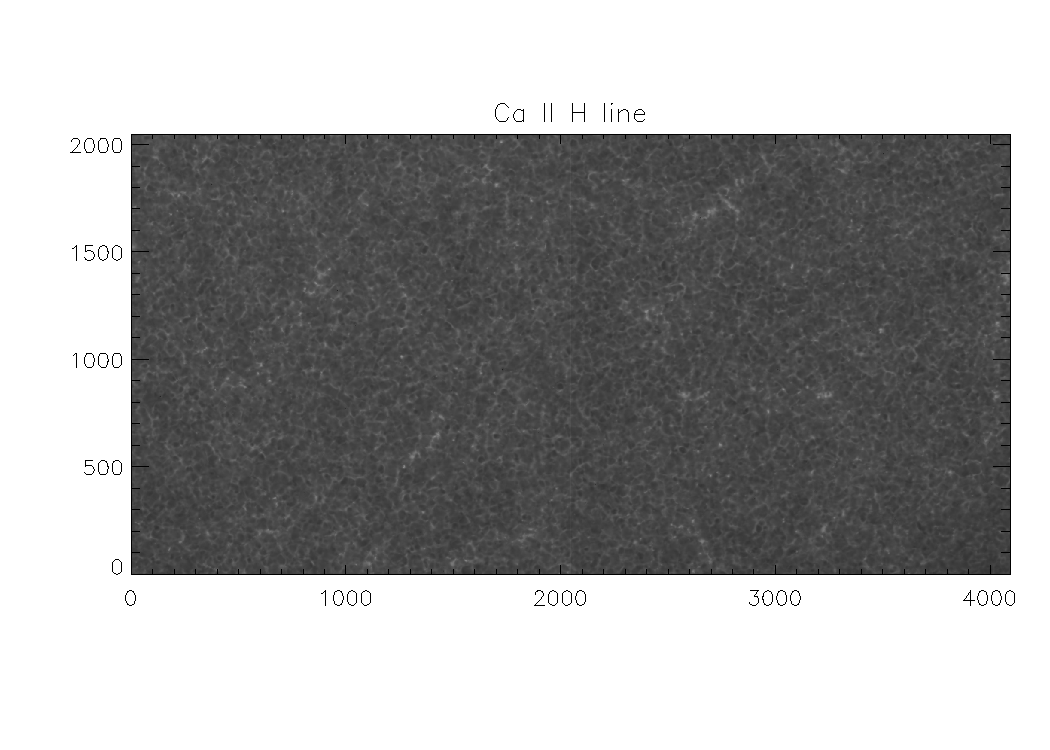
\includegraphics[width=\linewidth]{file4.pdf}
\end{figure}

\begin{figure}[H]
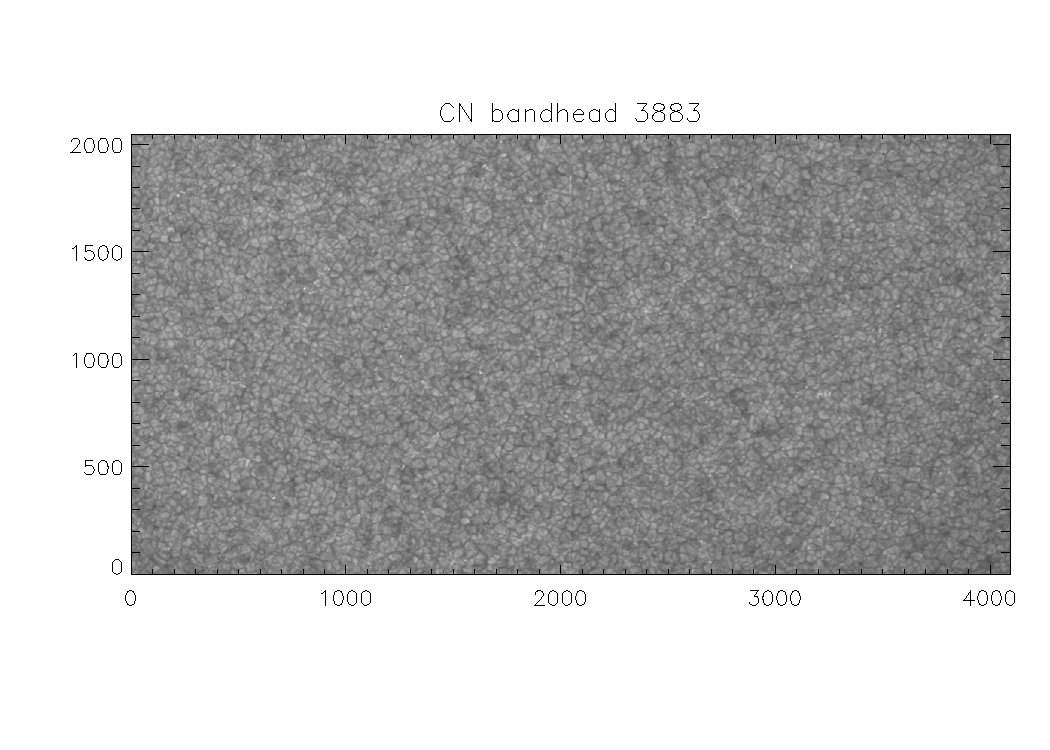
\includegraphics[width=\linewidth]{file5.pdf}
\end{figure}

\end{document}          
